
\documentclass{article}
\usepackage[margin=1in]{geometry}
\usepackage{amsmath}
\usepackage{amssymb}
\usepackage{graphicx}
\usepackage{float}


\begin{document}
\title{A guide for Bayesian analysis in ADMB}
\author{Cole C. Monnahan | monnahc@uw.edu}
\date{\today{}}
\maketitle
\begin{abstract}
  The point of this document is.....
\end{abstract}

\tableofcontents
\section{Bayesian inference}
A short intro with citations to better papers. Maybe merge
in what is currently shown?
\section{MCMC}
Markov chain Monte Carlo (MCMC) is a common algorithm used
to sample from arbitrary, unscaled posterior
distributions. ADMB implements two different MCMC
algorithms: the ubiqitous Metropolis-Hastings and a
Hamiltonian (or ``hybrid'') sampler, both described briefly
below.

All MCMC algorithms work by proposing new states
(i.e. parameter vectors) and moving to that state, or not,
depending on its density relative to the current state. The
algorithm thus generates series of autocorrelated parameter
vectors which can be thinned to produce independent samples
from the posterior distribution of interest.

\subsection{Workflow}
The following steps outline the basic workflow typically
used for conducting a MCMC in ADMB.
\begin{enumerate}
\item Build, run, and verify an ADMB model. This model must
  explicitly include the contribution of the priors to the
  objective function, such that the ADMB estimate is the
  posterior mode, rather than a maximum likelihood estimate.
\item Run an MCMC using the command line argument
  \texttt{-mcmc $N$ -mcsave $N_{\text{save}}$} (among other
  options, see below). The thinned draws are discarded,
  leaving a total of $N_{\text{out}}=N/N_{\text{save}}$
  saved draws. For example \texttt{-mcmc 1e6 -mcsave 1000}
  will run 1 million draws but only save (i.e.``thin'')
  every 1000th, for a total kept of $Nout=1000$.
\item After completion, run the model again with argument
  \texttt{-mceval}. This command tells ADMB to loop through
  the saved iterations (in the \texttt{.psv} file) and
  execute in the \texttt{mceval\_phase()}.
\item Pull results into R or other program to ensure the
  sample is sufficiently thinned, either visually or with
  tools using, for example, the \texttt{CODA} package.
\item If necessary, rerun the chain with more thinning, drop
  the first part of the chain as a ``burn-in,'' or run
  longer for more iterations.
\item Make whatever Bayesian inference is desired using the
  $Nout$ independent samples.
\end{enumerate}

\subsection{MCMC Phases}
ADMB is designed with two phases that are used to produce
MCMC output: (1) the \texttt{mcmc} phase and (2)
\texttt{mceval} phase. While the use of these phases is not
common (is this true??) among other MCMC software, and may
be a source of confusion for new ADMB users, they provide a
powerful and efficient framework for MCMC analyses.

The \texttt{mcmc} phase is the one with which most people
are already familiar. This is where ADMB generates new
parameter sets by proposing a set, and then determining
whether to move there or stay at the current set. This
process is repeated $N$ times, and how sets are proposed
depend on the algorithm used (see section \ref{sec:MH} and
\ref{sec:hybrid}). During this phase, the $Nout$ saved
parameter values are written to a \texttt{.psv} file
(described below). Note that if \texttt{-mcsave $nsave$} is
not specified, ADMB will run the MCMC but no values will be
saved.

The \texttt{mceval} is an optional phase that is designed to
be run after the \texttt{.psv} file has been
produced. During this phase, ADMB loops through the $Nout$
parameter combinations in the \texttt{.psv} file and reruns
the \texttt{PROCEDURE\_SECTION} in the \texttt{mceval()}
phase. This phase is extremely powerful because it allows
the user to minimize wasted calculations by parsing
calculations into two groups: those that affect the
objective function (i.e. posterior calculations for Bayesian
analyses) and those that do not. Calculations done for
discarded draws (which often is most iterations) simply slow
down the analysis. Thus, an analysis can be made to run
faster by minimizing calculations in the \texttt{mcmc}
phase.  For example, a user may want to extrapolate
(e.g. project a time series into the future) or calculate
values derived from the parameters and intermediate
values. By putting these calculations inside an
\texttt{mceval\_phase} clause they are only done for saved
draws and the MCMC will run faster. In practice, some chains
need to be thinned significantly more than 1 in 1000, so the
time saved can be substantial, especially if the
\texttt{mceval\_phase} calculations are time-consuming.

While the \texttt{mceval} phase was designed specifically
for MCMC analyses, it can be coopted for use in other types
of analyses. In essence it is a convenient framework in
which to get ADMB to quickly evaluate arbitrary sets of
parameters, while only initializing once. Examples of
alternative uses are the SIR algorithm (\ref{sec:sir}),
evaluating a grid of points for plotting and exploration of
the posterior surface, or trying random parameter sets to
investigate local minima. Getting ADMB to evaluate these
parameter sets is as simple as writing them to the
\texttt{.psv} file and then executing ADMB with the option
\texttt{-mceval}. See section (\ref{sec:outfiles}) for
details on how to do this.


\subsection{Output files}\label{sec:outfiles}
\subsubsection{Meta data: The hst file}
\subsubsection{Parameter draws: The psv file}
During the \texttt{mcmc} phase, saved parameter values, in
bounded space, are written to a binary file called
\texttt{<model name>.psv}. This file can be read into R
using the following commands:
\begin{verbatim}
psv <- file("<model name>.psv", "rb") 
nparams <- readBin(psv, "integer", n=1)
mcmc <- matrix(readBin(psv, "numeric", n=nparams*Nout), ncol=nparams, byrow=TRUE)
close(psv)
\end{verbatim}
The first element in the \texttt{.psv} file is the number of
active parameters in the model, which then tells R how to
parse the following elements into parameter values. Note
that the value of $Nout$ in \texttt{nparams*Nout} depends on
\texttt{Nmcmc} and \texttt{mcsave} and must be specified
manually. This is the main file that was designed to be used
to extract MCMC draws from ADMB. However, this file only
contains parameter values and not derived quantities or
other quantities of interest (e.g. $MSY$ or biomass
trajectories) which often are of interest. 
\subsubsection{Derived quantity draws}

A simple way of extracting this information is to bypass the
\texttt{psv} file altogether and use a \texttt{C++} function
to write a \texttt{.csv} file containing whatever elements
are desired. This can be accomplished inside the ADMB
\texttt{.tpl} file with just a few lines of code. Inside the
\texttt{DATA\_SECTION} section use the following code to
create an IO object that writes values to a \texttt{.csv}
file, similar to the function \texttt{cout} which prints to
screen.
\begin{verbatim}
 !!CLASS ofstream MCMCreport("MCMCreport.csv",ios::app);
\end{verbatim}
Then, inside the \texttt{PROCEDURE\_SECTION} the function
can be used to write both parameters, derived quantities, or
other information about the model.
\begin{verbatim}
  if(mceval_phase()){
    if(header==1) {
        MCMCreport << "a,b,NLL,ab" << endl;
        header=0;
    }
   MCMCreport << a <<"," << b << "," << NLL << "," << ab << endl;
  }
\end{verbatim}
The \texttt{MCMCreport} object is used just like
\texttt{cout} and is executed only during the
\texttt{mceval} phase so that only saved values are written
to the file. Naturally this code can be used anywhere in the
procedure section, and this may be a useful diagnostic tool
in some situations. New draws are appended to the
\texttt{MCMCreport.csv} file so that it must be deleted in
between MCMC runs.

\subsection{Restarting a chain}\label{sec:restart}
How to restart a chain if you need more samples. How does this work?
\subsection{Convergence diagnostics} \label{sec:diag}
Burn-in and thinning, how to check this? What happens if not
independent? 
\subsection{Starting values and scaling}\label{sec:startvals}
Where the algorithm starts from (MLE) and the scaling process
(default and user options). Must discard these draws!
\subsection{Metropolis-Hastings}\label{sec:MH}
The default MCMC algorithm used by ADMB is the
Metropolis-Hastings (MH) algorithm. This algorithm has been
around for decades, is simple to implement and used widely.

This algorithm will be most efficient when the posterior
surface mimics a multivariate Normal distribution.

\subsubsection{Algorithm}
Let
\begin{align*}
  f&=\text{the ADMB objective function}\\
  c&=\text{an unknown normalization constant}\\
  Xcur&=\text{current parameter vector}\\
  Xprop&=\text{a proposed parameter vector}\\
  U&=\text{a randomly drawn uniform value in [0,1]}\\
\end{align*}
Then
\begin{equation}
  Xnew=
  \begin{cases}
    Xprop & \text{if} \quad U\leq \dfrac{cf(Xprop)}{cf(Xcur)}\\
    Xcur & \text{otherwise}
  \end{cases}
\end{equation}
The proposal (or ``jump'') function proposes new parameter
vectors given the current set. The default behavior for ADMB
is to use a multivariate normal
distribution\footnote{Technically a bounded multivariate
  normal} centered at the current vector:
\begin{equation*}
  Xprop\sim MVN(Xcur, \Sigma)
\end{equation*}
 where $\Sigma$ is the covariance matrix obtained by
 inverting the Hessian at the posterior mode. 

In ADMB there are options to modify the proposal function to
achieve better efficiency.

\subsubsection{MCMC Arguments}
\begin{table}[h]
  \centering
  \begin{tabular}[h]{|cl|}
    \hline
    \texttt{-mcmc N} & Run $N$ MCMC iterations\\
    \texttt{-mcsave N} & Save every $N$th MCMC iterations\\
    \texttt{-mcscale N} & Rescale step size for first $N$ iterations\\
    \hline
  \end{tabular}
  \caption{ADMB runtime arguments for Metropolis-Hastings MCMC}
  \label{tab:mh_args}
\end{table}
\subsubsection{mcprobe}

\subsubsection{mcrb}
The \texttt{-mcrb N} option (which stands for rescaled
bounded) alters the covariance matrix used to propose new
parameter sets in the MH algorithm. Its intended use is to
create a more efficient MCMC sampler so the analyses run
faster. 

The option will be most effective under circumstances where
the correlation between parameters at the MPD is higher than
other regions of the parameter space. In this case, the
algorithm may make efficient proposals at the MPD, but
inefficient proposals in other parts of the space. By
reducing the correlation using \texttt{mcrb} the proposal
function may be more efficient on average across the entire
parameter space and require less thinning.


The \texttt{mcrb} option is a set of calculations performed
on the original correlation matrix, as follows.
\begin{align*}
  \mathbf{\Sigma_{\text{old}}}&=
  \begin{bmatrix}
    1 & \cdots & \rho_{1,n}\\
    \vdots & \ddots & \vdots\\
    \rho_{n,1} & \cdots & 1
  \end{bmatrix}
  \quad\text{The original correlation matrix}\\
  \mathbf{L}&=\begin{bmatrix}
    1 & \cdots & 0\\
    \vdots & \ddots & \vdots\\
    L_{n,1} & \cdots & L_{n,n}
  \end{bmatrix}
  \quad\text{Lower Choleski decomposition of $ \mathbf{\Sigma_{\text{old}}}$}\\
  \mathbf{\hat{L}}&=\begin{bmatrix}
    1 & \cdots & 0\\
    \vdots & \ddots & \vdots\\
    L_{n,1}^{N/10} & \cdots & L_{n,n}^{N/10}
  \end{bmatrix}
  \quad\text{Raise elements to power user supplied $N$}\\
  \mathbf{\tilde{L}}&=\begin{bmatrix}
    1 & \cdots & 0\\
    \vdots & \ddots & \vdots\\
    \frac{\hat{L}_{n,1}}{\left | \hat{L}_{n,\cdot}\right |} & \cdots &
    \frac{\hat{L}_{n,n}}{\left | \hat{L}_{n,\cdot}\right |}
  \end{bmatrix}
  \quad\text{Normalize rows of $\hat{L}$ }\\
  \mathbf{\Sigma_{\text{rb}}}&=\mathbf{\tilde{L}}\mathbf{\tilde{L}}^T
  \quad\text{Calculate new correlation matrix}
\end{align*}

By working with the Choleski decomposition of the
correlation matrix, the algorithm ensures that the rescaled
bounded matrix used in the MCMC remains a valid correlation
matrix (i.e. positive definite).

\begin{figure}[h]
  \centering
  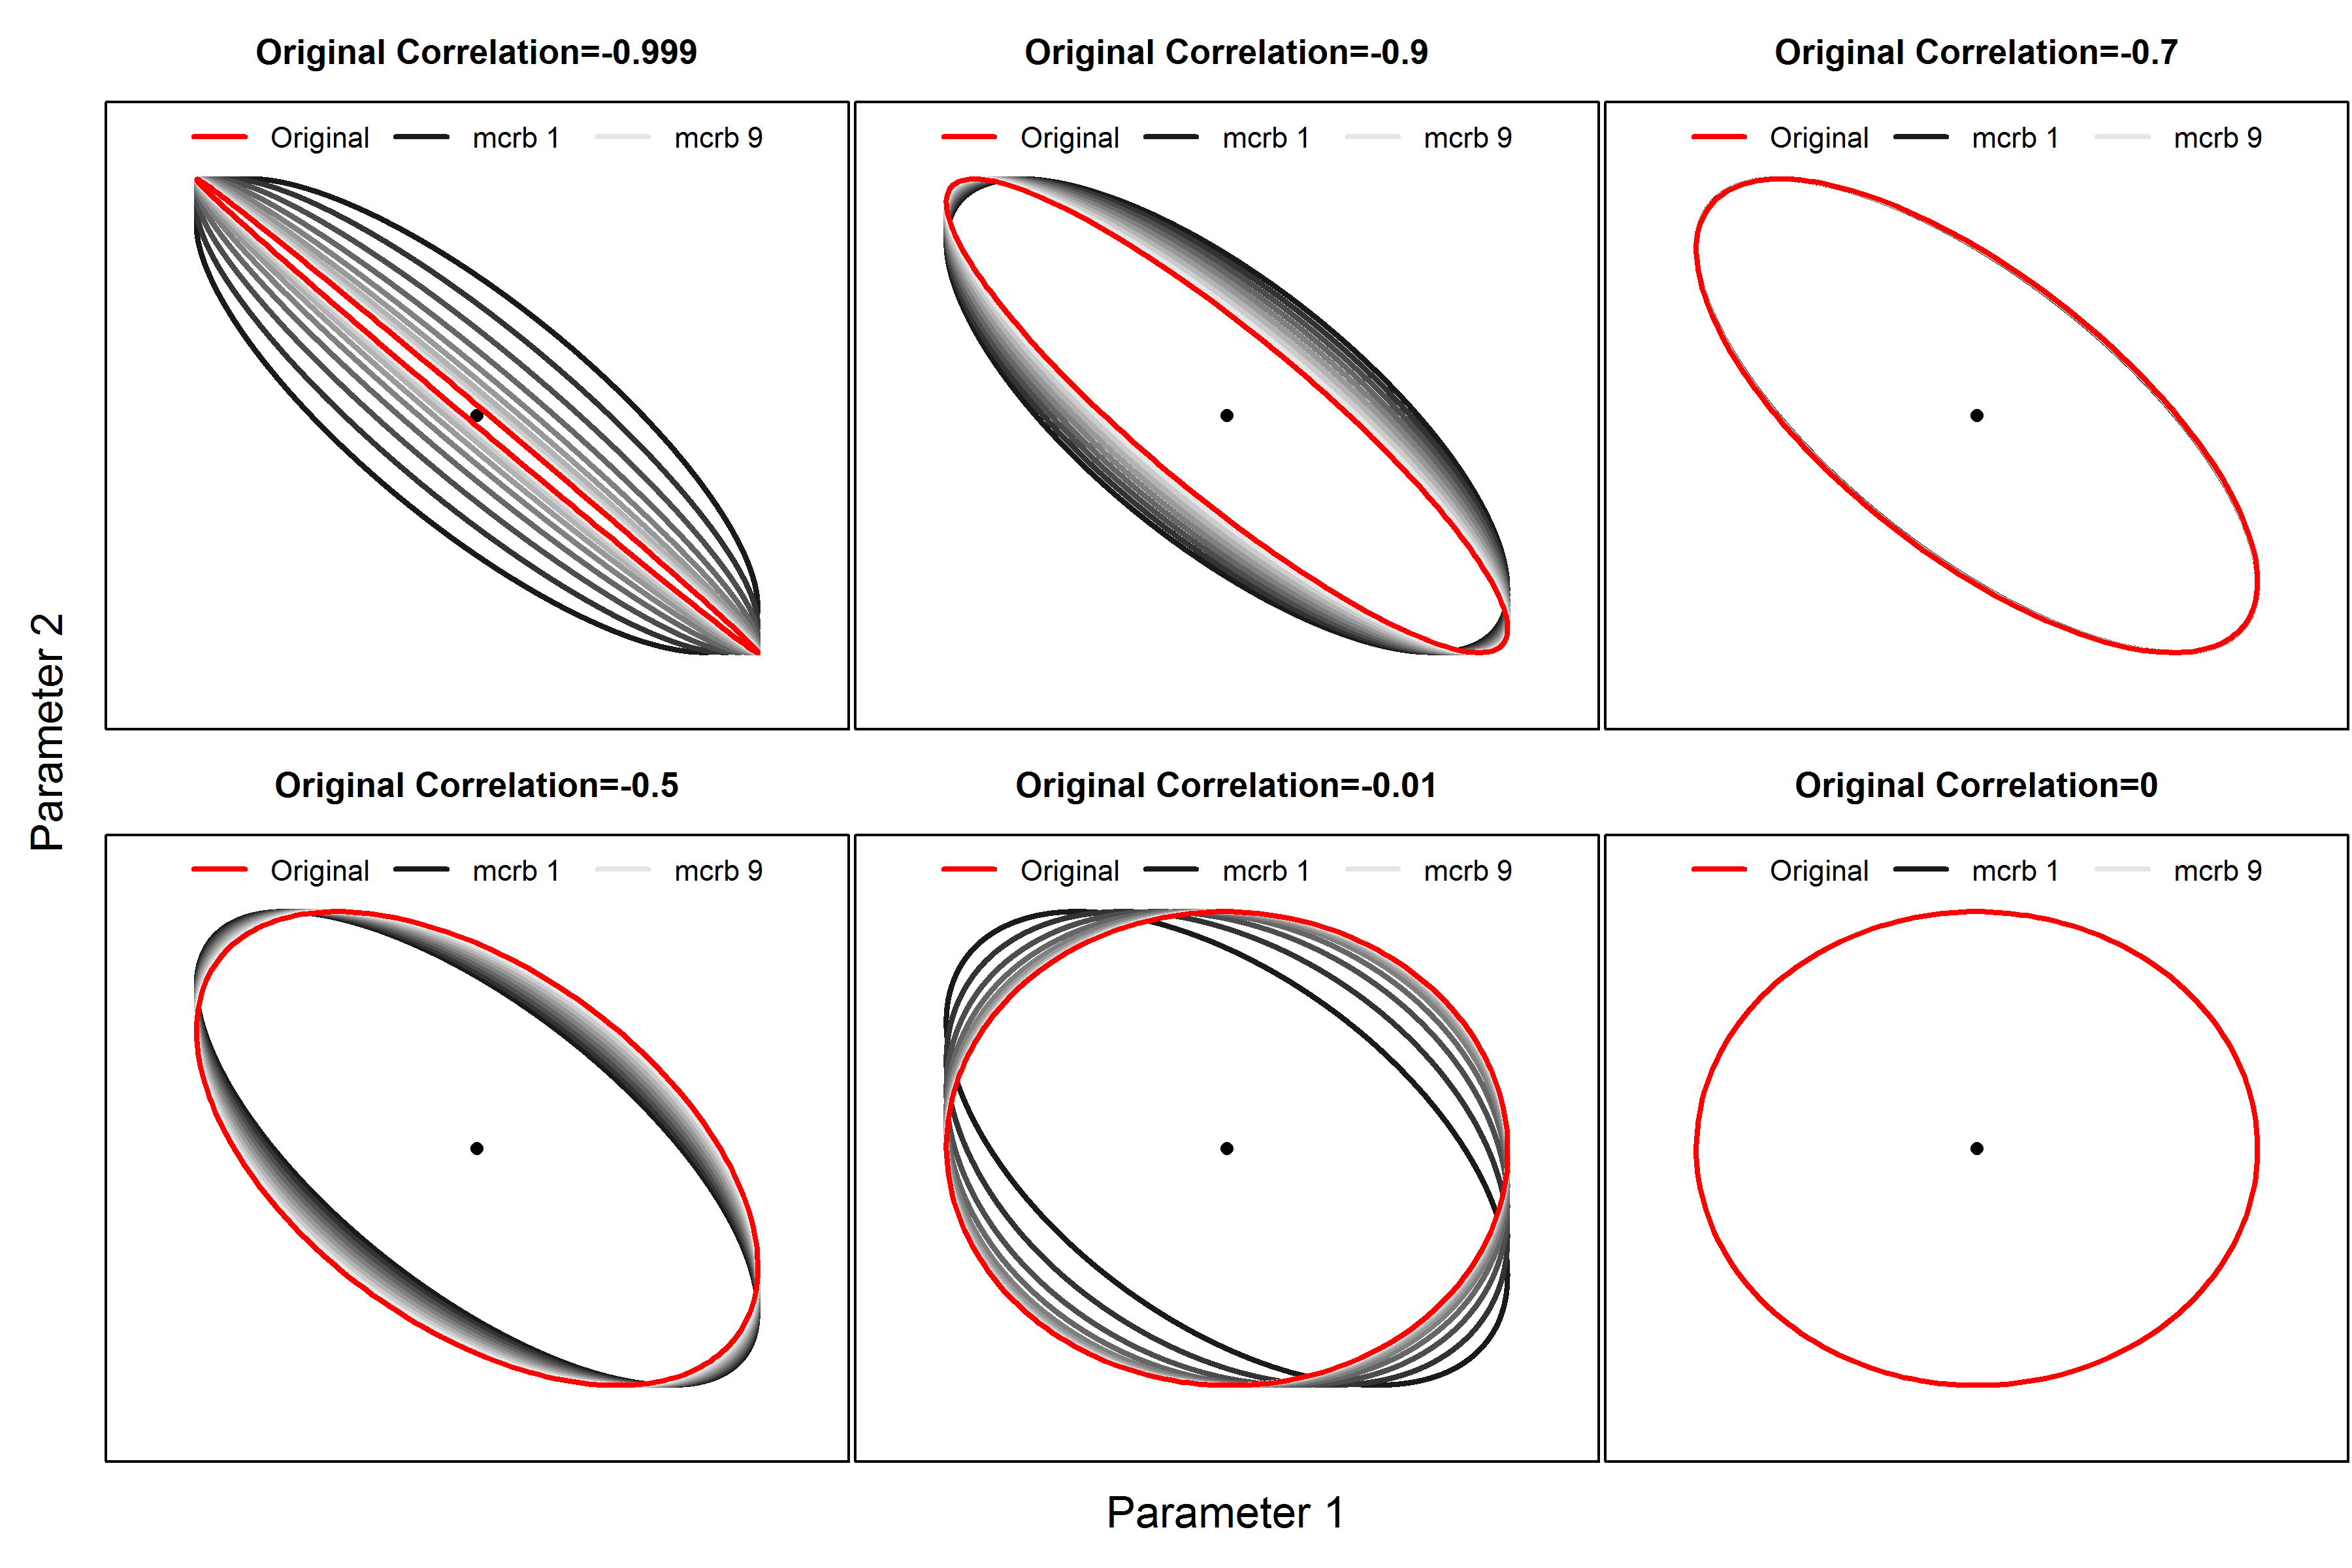
\includegraphics[width=5in]{plots/mcrb_examples.png}
  \caption{The effect of \texttt{mcrb} on a variety of
    correlations between two hypothetical parameters. Note
    that the effect of setting $N=9$ depends on the original
    correlation.}
  \label{fig:mcrb}
\end{figure}
\subsubsection{User-supplied correlation matrix}
If the MLE covariance is inefficient at proposing. Why do this?
How? Show code for how to do this, and talk about positive
definitness.
\subsubsection{Example MCMC}
Use a simple model to demonstrate some of these
concepts. Especially the workflow and examining convergence
properties, but also maybe restarting.
\subsection{Hyrbid}\label{sec:hybrid}
\subsubsection{Algorithm}
Quick explanation of this.
\subsubsection{Arguments}
Only show those different than the MH algorithm.
\section{SIR}\label{sec:sir}
\subsubsection{Algorithm}
\subsubsection{Example}
Use same model as the other example and show how to do SIR in R,
then compare the two posteriors to show the same.
\section{Running analyses in R}
How to create top-level functions for running analyses
programmatically.
\subsection{Code}
Here is one I wrote for my thesis, which could be generalized
easily. Use psv file here, or force user to write to csv? Let
them use append or always overwrite files? Who actually restarts?
\begin{verbatim}
run.mcmc <- function(Nout, mcsave, burn.in, boot, cor.mat=NULL, init.pin=NULL,
                     se.scale=NULL, mcscale=FALSE, mcdiag=FALSE, mcseed=NULL,
                     mcrb=NULL, mcgrope=NULL, verbose=TRUE, extra.args=NULL){
    ## This function runs an ADMB model MCMC, burns and thins, calculates
    ## effective sizes, and returns stuff depending on verbose.
    require(coda)
    model <- "logistic"
    thin.every <- 1                     # setting to 1 for this project
    iterations <- (Nout+burn.in)*mcsave
    ##    print(paste("Run started at", round(Sys.time())))
    if(iterations <1) stop(paste0("Iterations too low: ", iterations))
    wd.old <- getwd(); on.exit(setwd(wd.old))
    setwd(model.dir)
    ## Run to get MLE and covariance matrix if none provided
    if(is.null(init.pin)) system(model, ignore.stdout=T) else {
        write.table(file="init.pin", x=init.pin, row.names=F, col.names=F)
    }

    if(!is.null(se.scale)) SetScale(se.scale) # change the covariance matrix
    ## Clean up the old files
    file.list <-c("mc_abundances.csv","mc_abundances_def.csv",
                  "mc_abundances_mit.csv", "mc_abundances_none.csv",
                  "mc_shipstrikes.csv", "mc_shipstrikes_def.csv",
                  "mc_shipstrikes_mit.csv", "mc_shipstrikes_none.csv",
                  "mc_parameters.csv", "mc_vessels.csv", "mc_equil.csv")
    suppressWarnings(file.remove(file.list))
    cmd <- paste(model,"-mcmc",iterations,"-nohess -noest")
    ## make the argument and run the MCMC
    if(!is.null(mcseed)) cmd <- paste(cmd, "-mcseed", mcseed)
    cmd <- paste(cmd, "-mcsave",mcsave)
    if(mcscale==FALSE) cmd <- paste(cmd, "-mcnoscale")
    if(!is.null(mcrb)) cmd <- paste(cmd, "-mcrb",mcrb)
    if(!is.null(mcgrope)) cmd <- paste(cmd, "-mcgrope",mcgrope)
    if(mcdiag==TRUE) cmd <- paste(cmd, "-mcdiag")
    if(!is.null(extra.args)) cmd <- paste(cmd, extra.args)
    if(!is.null(init.pin)) cmd <- paste(cmd, "-mcpin init.pin")
    ##  print(cmd)
    ## If user provided covar matrix, write it to file
    if(!is.null(cor.mat)) writeADMBCovariance(cor.mat)
    system(cmd, ignore.stdout=T)
    system(paste(model, "-mceval -noest -nohess"), ignore.stdout=T)

    ## Read in the results
    df <- read.csv("mc_parameters.csv")
    vessels <- read.csv("mc_vessels.csv", head=T)
    S <- read.csv("mc_shipstrikes.csv")
    S.none <- read.csv("mc_shipstrikes_none.csv")
    S.mit <- read.csv("mc_shipstrikes_mit.csv")
    S.def <- read.csv("mc_shipstrikes_def.csv")
    N <- read.csv("mc_abundances.csv")
    N.none <- read.csv("mc_abundances_none.csv")
    N.mit <- read.csv("mc_abundances_mit.csv")
    N.def <- read.csv("mc_abundances_def.csv")
    D <- N/df$K
    D.none <- N.none/df$K
    D.mit <- N.mit/df$K
    D.def <- N.def/df$K
    equil <- read.csv("mc_equil.csv")
    ## Rows are mcmc iterations, cols are years except df which is parameters
    mcmc <- list(params=df, vessels=vessels, S=S, D=D, N=N,
                 S.none=S.none, S.mit=S.mit, S.def=S.def,
                 N.none=N.none, N.mit=N.mit, N.def=N.def,
                 D.none=D.none, D.mit=D.mit, D.def=D.def,
                 equil=equil)
    if(nrow(df)>burn.in) mcmc <- lapply(mcmc, function(x) x[-(1:burn.in),])
    else stop ("Too few samples to thin/burn")
    ## Run effective sample size calcs from CODA, metric of convergence
    efsize <- data.frame(t(effectiveSize(df)/nrow(df)))
    names(efsize) <- paste0(names(df), "_efs")
    ## Grab admb fit and metrics
    fit <- read.admbFit("logistic")
    mle <- with(fit,
                data.frame(NLL=nloglike, maxgrad=maxgrad,
                           rMSY.cor=cor[2,1], boot=boot))
    temp <- data.frame(t(fit$est), row.names=F)
    names(temp) <- paste0(fit$names, "_mle")
    mle <- cbind(mle, temp[,-ncol(temp)])
    temp <- data.frame(t(fit$std), row.names=F)
    names(temp) <- paste0(fit$names, "_se")
    mle <- cbind(mle, temp[,-ncol(temp)])
    fit.df <- cbind(mle, efsize)
    if(verbose) return(list(fit.df=fit.df, mcmc=mcmc))
    else return(fit.df=fit.df)
}
\end{verbatim}

\end{document}




